%
\documentclass[10pt,a4paper]{article}


\usepackage{array}
\usepackage{subfigure}
\usepackage{graphicx}
\usepackage{amssymb}
\usepackage{amsmath}
\usepackage{cite}
\usepackage{color}
\usepackage{url}
\usepackage[lined,linesnumbered,ruled,norelsize]{algorithm2e}
\usepackage{listings}

\begin{document}

\title{Experiment 5: Naive Bayes}

\maketitle
  
\section{Description}
%
  In this exercise, you will use Naive Bayes to classify email messages into spam and nonspam groups. Your dataset is a preprocessed subset of the Ling-Spam Dataset, provided by Ion Androutsopoulos. It is based on 960 real email messages from a linguistics mailing list.

  There are two ways to complete this exercise. The first option is to use the Matlab/Octave-formatted features we have generated for you. This requires using Matlab/Octave to read prepared data and then writing an implementation of Naive Bayes. To choose this option, download the data pack ex5DataPrepared.zip.

  The second option is to generate the features yourself from the emails and then implement Naive Bayes on top of those features. You may want this option if you want more practice with features and a more open-ended exercise. To choose this option, download the data pack ex5DataEmails.zip.








\section{Data}
%

  The dataset you will be working with is split into two subsets: a 700-email subset for training and a 260-email subset for testing. Each of the training and testing subsets contain 50\% spam messages and 50\% nonspam messages. Additionally, the emails have been preprocessed in the following ways:
  %
  \begin{enumerate}
    \item Stop word removal: Certain words like ``and'', ``the'', and ``of'', are very common in all English sentences and are not very meaningful in deciding spam/nonspam status, so these words have been removed from the emails.
    %
    \item Lemmatization: Words that have the same meaning but different endings have been adjusted so that they all have the same form. For example, ``include'', ``includes'', and ``included'', would all be represented as ``include''. All words in the email body have also been converted to lower case.
    %
    \item Removal of non-words: Numbers and punctuation have both been removed. All white spaces (tabs, newlines, spaces) have all been trimmed to a single space character.
  \end{enumerate}

  As an example, here are some messages before and after preprocessing:

  \vspace{2ex}
  \textbf{Nonspam message ``5-1361msg1'' before preprocessing}
  %
  \begin{lstlisting}[language=C, basicstyle=\footnotesize, showspaces=false]
    Subject: Re: 5.1344 Native speaker intuitions
  
    The discussion on native speaker intuitions has been extremely
    interesting, but I worry that my brief intervention may have
    muddied the waters. I take it that there are a number of
    separable issues. The first is the extent to which a native
    speaker is likely to judge a lexical string as grammatical
    or ungrammatical per se. The second is concerned with the
    relationships between syntax and interpretation (although even
    here the distinction may not be entirely clear cut).
  \end{lstlisting}



  \vspace{2ex}
  \textbf{Nonspam message ``5-1361msg1'' after preprocessing}
  %
  \begin{lstlisting}[language=C, basicstyle=\footnotesize, showspaces=false]
    re native speaker intuition discussion native speaker intuition 
    extremely interest worry brief intervention muddy waters number 
    separable issue first extent native speaker likely judge lexical 
    string grammatical ungrammatical per se second concern relationship 
    between syntax interpretation although even here distinction entirely clear cut
  \end{lstlisting}


  \vspace{2ex}
  %
  For comparison, here is a preprocessed spam message.


  \vspace{2ex}
  \textbf{Spam message ``spmsgc19'' after preprocessing}
  %
  \begin{lstlisting}[language=C, basicstyle=\footnotesize, showspaces=false]
    financial freedom follow financial freedom work ethic extraordinary 
    desire earn least per month work home special skills experience 
    required train personal support need ensure success legitimate 
    homebased income opportunity put back control finance life ve 
    try opportunity past fail live promise
  \end{lstlisting}

  As you can discover from browsing these messages, preprocessing has left occasional word fragments and nonwords. In the end, though, these details do not matter so much in our implementation (you will see this for yourself).




\section{Multinomial Naive Bayes}
%
  To classify our email messages, we will use a multinomial Naive Bayes model. The parameters of our model are as follows:
  %
  %
  \begin{figure}[htb!]
    \centering
      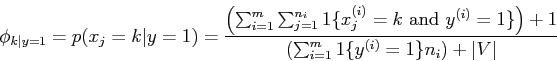
\includegraphics[width=.8\columnwidth]{img1} \\
      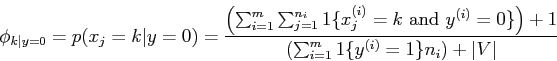
\includegraphics[width=.8\columnwidth]{img2} \\
      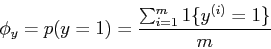
\includegraphics[width=.4\columnwidth]{img3}
  \end{figure}
  %
  Recall that
  %
  \begin{itemize}
    \item $\phi_{k\vert y=1}$ estimates the probability that a particular word in a spam email will be the $k$-th word in the dictionary
    \item $\phi_{k\vert y=0}$ estimates the probability that a particular word in a nonspam email will be the $k$-th word in the dictionary
    \item $\phi_{y}$ estimates the probability that any particular email will be a spam email
  \end{itemize}
  %
  Here are some other notation conventions:
  %
  \begin{itemize}
    \item $m$ is the number of emails in our training set
    \item The $i$-th email contains $n_{i}$ words.
    \item The entire dictionary contains $\vert V\vert$ words
  \end{itemize}
  %

  You will calculate the parameters $\phi_{k\vert y=1}$, $\phi_{k\vert y=0}$, and $\phi_{y}$ from the training data. Then, to make a prediction on an unlabeled email, you will use the parameters to compare  $p(x\vert y=1)p(y=1)$ and  $p(x\vert y=0)p(y=0)$, as described in the lecture videos. In this exercise, instead of comparing the probabilities directly, it is better to work with their logs. That is, you will classify an email as spam if you find
  %
  \begin{displaymath}
    \log p(x\vert y=1)+\log p(y=1)>\log p(x\vert y=0)+\log p(y=0)
  \end{displaymath}


\section{Implementing Naive Bayes Using Prepared Features}
%
  If you want to complete this exercise using the formatted features we provided, follow the instructions in this section.

  In the data pack for this exercise, you will find a text file named ``train-features.text'' that contains the features of emails to be used in training. The lines of this document have the following form:
  %
  \begin{lstlisting}[language=C, basicstyle=\footnotesize, showspaces=false]
    2 977 2
    2 1481 1
    2 1549 1
  \end{lstlisting}

  The first number in a line denotes a document number, the second number indicates the ID of a dictionary word, and the third number is the number of occurrences of the word in the document. So in the snippet above, the first line says that Document 2 has two occurrences of word 977.

  To look up what word 977 is, use the ``feature-tokens.txt'' file, which lists each word in the dictionary alongside an ID number.



  \subsection{Load The Features}
  %
  Now load the training set features into Matlab/Octave in the following way:
  %
  \begin{lstlisting}[language=Octave, basicstyle=\footnotesize, showspaces=false]
    numTrainDocs = 700;
    numTokens = 2500;
    M = dlmread('train-features.txt', ' ');
    spmatrix = sparse(M(:,1), M(:,2), M(:,3), numTrainDocs, numTokens);
    train_matrix = full(spmatrix);
  \end{lstlisting}
  %
  This loads the data in our ``train-features.txt'' into a sparse matrix (a matrix that only stores information for non-zero entries). The sparse matrix is then converted into a full matrix, where each row of the full matrix represents one document in our training set, and each column represents a dictionary word. The individual elements represent the number of occurrences of a particular word in a document.


  For example, if the element in the $i$-th row and the $j$-th column of train\_matrix contains a ``4'', then the $j$-th word in the dictionary appears 4 times in the $i$-th document of our training set. Most entries in train\_matrix will be zero, because one email includes only a small subset of the dictionary words.

  Next, we'll load the labels for our training set.
  %
  \begin{lstlisting}[language=Octave, basicstyle=\footnotesize, showspaces=false]
    train_labels = dlmread('train-labels.txt');
  \end{lstlisting}
  %
  This puts the $y$-labels for each of the $m$ the documents into an $m \times 1$ vector. The ordering of the labels is the same as the ordering of the documents in the features matrix, i.e. the $i$-th label corresponds to the $i$-th row in train\_matrix.



  \subsection{A Note on The Features}
  %
  In a Multinomial Naive Bayes model, the formal definition of a feature vector $\vec{x}$ for a document says that $x_j = k$ if the j-th word in this document is the k-th word in the dictionary. This does not exactly match our Matlab/Octave matrix layout, where the j-th term in a row (corresponding to a document) is the number of occurrences of the j-th dictionary word in that document.

  Representing the features in the way we have allows us to have uniform rows whose lengths equal the size of the dictionary. On the other hand, in the formal Multinomial Naive Bayes definition, the feature  $\vec{x}$ has a length that depends on the number of words in the email. We've taken the uniform-row approach because it makes the features easier to work with in Matlab/Octave.

  Though our representation does not contain contain any information about the position within an email that a certain word occupies, we do not lose anything relevant for our model. This is because our model assumes that each $\phi_{k\vert y}$ is the same for all positions of the email, so it's possible to calculate all the probablities we need without knowing about these positions.



  \subsection{Training}
  %
  You now have all the training data loaded into your program and are ready to begin training your data. Here are the recommended steps for proceeding:
  %
  \begin{enumerate}
    \item Calculate $\phi_{y}$
    \item Calculate each  $\phi_{k\vert y=1}$ for each dictionary word and store the all results in a vector.
    \item Calculate each  $\phi_{k\vert y=0}$ fore each dictionary word store the all results in a vector.
  \end{enumerate}



  \subsection{Testing}
  %
  Now that you have calculated all the parameters of the model, you can use your model to make predictions on test data. If you are putting your program into a script for Matlab/Octave, you may find it helpful to have separate scripts for training and testing. That way, after you've trained your model, you can run the testing independently as long as you don't clear the variables storing your model parameters.

  Load the test data in ``test-features.txt'' in the same way you loaded the training data. You should now have a test matrix of the same format as the training matrix you worked with earlier. The columns of the matrix still correspond to the same dictionary words. The only difference is that now the number of documents are different.

  Using the model parameters you obtained from training, classify each test document as spam or non-spam. Here are some general steps you can take:
  %
  \begin{enumerate}
    \item For each document in your test set, calculate  $\log p(\vec{x} \vert y = 1) + \log p(y=1)$
    \item Similarly, calculate  $\log p(\vec{x} \vert y = 0) + \log p(y=0)$
    \item Compare the two quantities from (1) and (2) above and make a decision about whether this email is spam. In Matlab/Octave, you should store your predictions in a vector whose i-th entry indicates the spam/nonspam status of the i-th test document.
  \end{enumerate}
  %
  Once you have made your predictions, answer the questions in the Questions section.
  



\section{Implementing Naive Bayes Without Prepared Features}
%
  Here are some guidelines that will help you if you choose to generate your own features. After reading this, you may find it helpful to read the previous section, which tells you how to work with the features.


  \subsection{Data Content}
  %
  The data pack you downloaded contains 4 folders.
  %
  \begin{itemize}
    \item[a] The folders ``nonspam-train'' and ``spam-train'' contain the preprocessed emails you will use for training. They each have 350 emails.
    \item[b] The folders ``nonspam-train'' and ``nonspam-test'' constitute the test set containing 130 spam and 130 nonspam emails. These are the documents you will make predictions on. Notice that even though the separate folders tell you the correct labeling, you should make your predictions on all the test documents without this knowledge. After you make your predictions, you can use the correct labeling to check whether your classifications were correct.
  \end{itemize}



  \subsection{Dictionary}
  %
  You will need to generate a dictionary for your model. There is more than one way to do this, but an easy method is to count the occurrences of all words that appear in the emails and choose your dictionary to be the most frequent words. If you want your results to match ours exactly, you should pick the dictionary to be the 2500 most frequent words.

  To check that you have done this correctly, here are the 5 most common words you will find, along with their counts.
  %
  \begin{lstlisting}[language=C, basicstyle=\footnotesize, showspaces=false]
    1. email 2172
    2. address 1650
    3. order 1649
    4. language 1543
    5. report 1384
  \end{lstlisting}
  %
  Remember to take the counts over all of the emails: spam, nonspam, training set, testing set.




  \subsection{Feature Generation}
  %
  Once you have the dictionary, you will need to represent your documents as feature vectors over the space of the dictionary words. Again, there are several ways to do this, but here are the steps you should take if you want to match the prepared features we described in the previous section.
  %
  \begin{enumerate}
    \item For each document, keep track of the dictionary words that appear, along with the count of the number of occurrences.
    \item Produce a feature file where each line of the file is a triplet of (docID, wordID, count). In the triplet, docID is an integer referring to the email, wordID is an integer referring to a word in the dictionary, and count is the number of occurrences of that word. For example, here are the first five entries of a training feature file we produced (the lines are sorted by docID, then by wordID):
    %
    \begin{lstlisting}[language=C, basicstyle=\footnotesize, showspaces=false]
      1 19 2
      1 45 1
      1 50 1
      1 75 1
      1 85 1
    \end{lstlisting}
  %
  \end{enumerate}

  In this snippet, Document 1 refers to the first document in the ``nonspam-train'' folder, ``3-380msg4.txt''. Our dictionary is ordered by the popularity of the words across all documents, so a wordID of 19 refers to the 19th most common word.

  This format makes it easy for Matlab/Octave to load your features as an array. Notice that this way of representing the emails does not contain any information about the position within an email that a certain word occupies. This is not a problem in our model, since we're assuming each $\phi_{k\vert y}$ is the same for all positions.



  \subsection{Training and Testing}
  %
  Finally, you will need to train your model on the training set and predict the spam/nonspam classification on the test set. For some ideas on how to do this, refer to the instructions in the previous section about working with already-generated features.

  When you are finished, answer the questions in the following Questions section.


\section{Question}
%
  \subsection{Classification Error}
  %
  Load the correct labeling for the test documents into your program. If you used the pre-generated features, you can just read ``test-labels.txt'' into your program. If you generated your own features, you will need to write your own labeling based on which documents were in the spam folder and which were in the nonspam folder.

  Compare your Naive-Bayes predictions on the test set to the correct labeling. How many documents did you misclassify? What percentage of the test set was this?


  \subsection{Smaller Training Sets}
  %
  Let's see how the classification error changes when you train on smaller training sets, but test on the same test set as before. So far you have been working with a 960-document training set. You will now modify your program to train on 50, 100, and 400 documents (the spam to nonspam ratio will still be one-to-one).

  If you are using our prepared features for Matlab/Octave, you will see text documents in the data pack named ``train-features-\#.txt'' and ``train-labels-\#.txt'', where the ``\#'' tells you how many documents make up these training sets. For each of the training set sizes, load the corresponding training data into your program and train your model. Then record the test error after testing on the same test set as before.

  If you are generating your own features from the emails, you will need to select email subsets of 50, 100, and 400, keeping each subset 50\% spam and 50\% nonspam. For each of these subsets, generate the training features as you did before and train your model. Then, test your model on the 260-document test set and record your classification error.







\end{document}
